\newcommand{\nom}{La cordeuse}
\input{../../headers/beamersystemesHeadings}

\section{Introduction}

{\frame{
\frametitle{D�marrer le syst�me}

\begin{enumerate}
 \item Allumer la cordeuse,
 \begin{center}
  \includegraphics[width=0.4\linewidth]{img/0001}
 \end{center}
  \item Allumer le boitier de mesure.
 \begin{center}
  \includegraphics[width=0.4\linewidth]{img/0002}
 \end{center}
\end{enumerate}
}}

{\frame{
\frametitle{Lancer le logiciel d'acquisition et effectuer une mesure}

\begin{enumerate}
 \item Cliquer sur le menu d�marrer et tapper \og SP55 \fg dans la barre de recherche,
 \begin{center}
  \includegraphics[width=0.3\linewidth]{img/0003}
 \end{center}
  \item Cliquer sur l'ic�ne \og Effectuer une mesure\fg,
 \begin{center}
  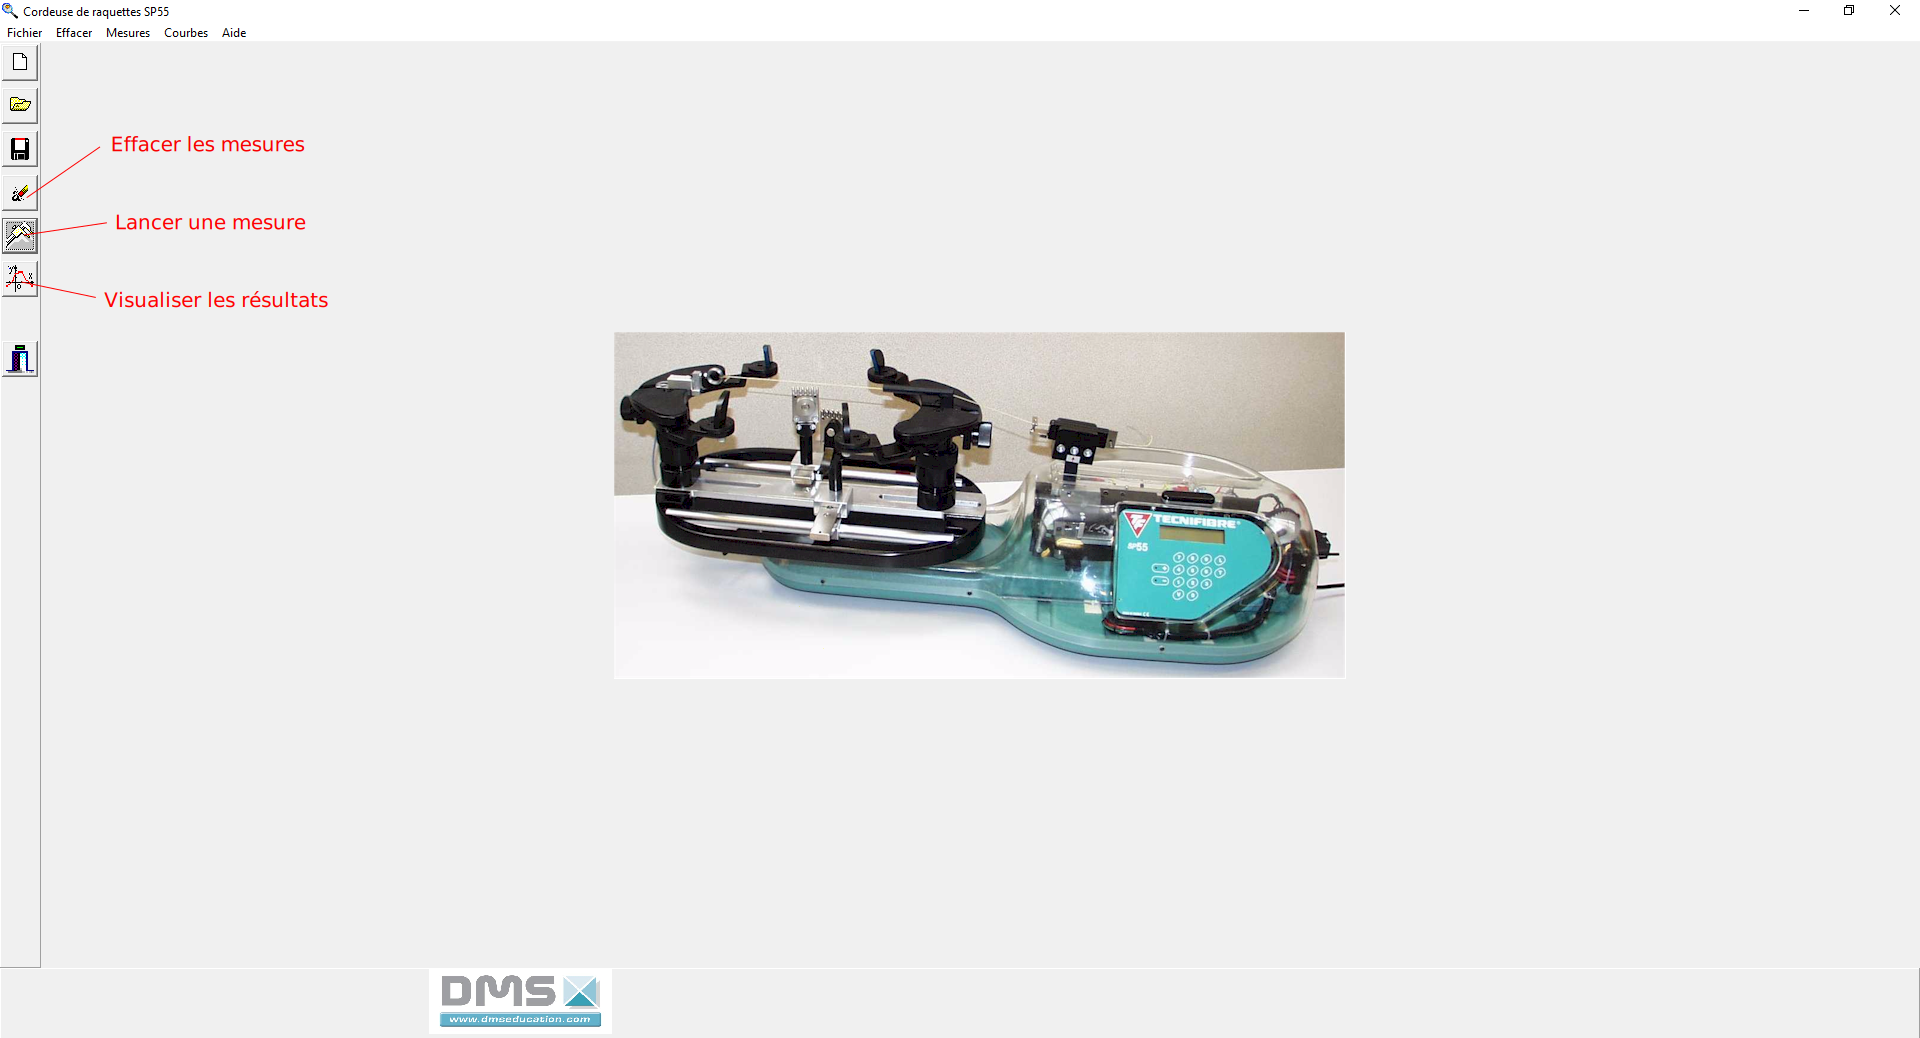
\includegraphics[width=0.3\linewidth]{img/0004}
 \end{center}
  \item Cliquer sur \og Initialiser \fg,
 \begin{center}
  \includegraphics[width=0.3\linewidth]{img/0005a}
 \end{center}
 \end{enumerate}
}}

{\frame{
\frametitle{Lancer le logiciel d'acquisition et effectuer une mesure}

\begin{enumerate}
\setcounter{enumi}{3}
 \item Appuyer sur le \og Bouton d�part \fg,
 \begin{center}
  \includegraphics[width=0.3\linewidth]{img/0006}
 \end{center}
  \item Lancer lamise sous tension de la corde,
 \begin{center}
  \includegraphics[width=0.3\linewidth]{img/0007}
 \end{center}
  \item Arr�ter cette mise sous tension par le m�me bouton,
  \end{enumerate}
}}

{\frame{
\frametitle{Lancer le logiciel d'acquisition et effectuer une mesure}

\begin{enumerate}
\setcounter{enumi}{6}
  \item A la fin de la mesure, les donn�es sont charg�es dans le logiciel,
 \begin{center}
  \includegraphics[width=0.3\linewidth]{img/0005}
 \end{center}
  \item Choisir la mesure � afficher,
 \begin{center}
  \includegraphics[width=0.1\linewidth]{img/0008}
 \end{center}
 \item Choisir parmis les ic�nes (1) la donn�e � afficher en abscisse et la.es donn�e.s � afficher en ordonn�e du graphique (2),
 \begin{center}
  \includegraphics[width=0.3\linewidth]{img/0008a}
 \end{center}
 \item Cliquer sur \og Tracer \fg (3).
 \end{enumerate}
}}

{\frame{
\frametitle{Eteindre le syst�me}

\begin{enumerate}
 \item �teindre le PC, 
 \item �teindre la cordeuse,
 \begin{center}
  \includegraphics[width=0.3\linewidth]{img/0001}
 \end{center}
  \item �teindre le boitier de mesure.
 \begin{center}
  \includegraphics[width=0.3\linewidth]{img/0002}
 \end{center}
\end{enumerate}
}}


\end{document}

